\section{System's Perspective}

\subsection{Design and Architecture}
Figure \ref{fig:systemoverview} provides an overview of our system infrastructure:
\begin{figure}[H]
    \centering
    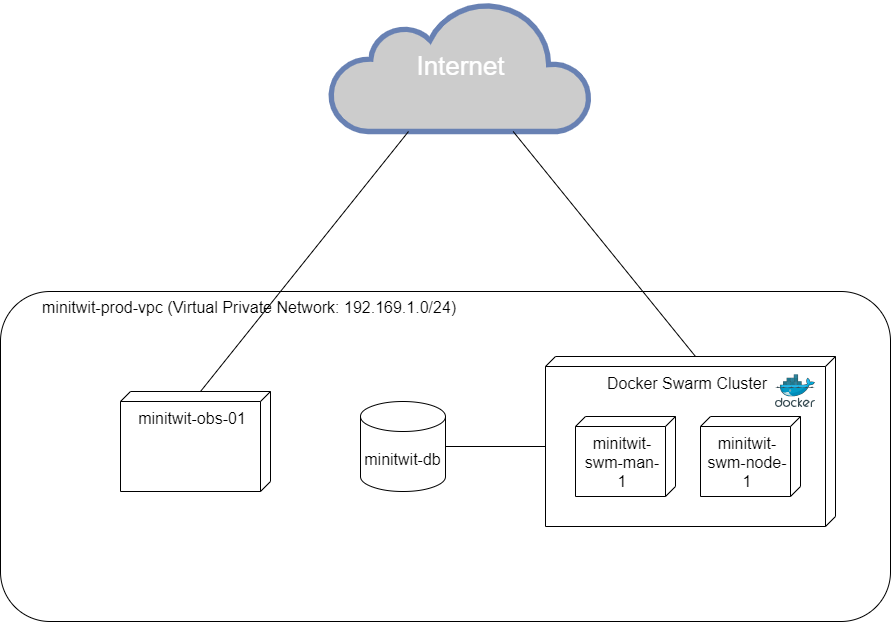
\includegraphics[width=0.7\linewidth]{images/system-overview3.png}
    \caption{Overview of the system}
    \label{fig:systemoverview}

\end{figure}
The system includes a single Virtual Private Network with an IP 192.168.1.0/24. Within this network, we operate a database cluster consisting of a single node. This node is connected to the Docker Swarm cluster, featuring both a manager and a worker node.

Both our monitoring and cluster servers are visibly exposed to the internet. Additionally, the database server is accessible from the internet but has constraints to only talk to our servers and therefore not accept requests from any other host.

\subsection{Interactions of Subsystems}
Our system consists of two main subsystems, namely the REST SimulatorAPI and the webapplication Minitwit. As can be seen in figure \ref{fig:subsystem-interaction}, The SimulatorAPI and Minitwit subsystems are similar in structure. However when looking at the processes behind the structures in Figure \ref{fig:frontend-interaction} and \ref{fig:backend-interaction} it is apparant that these two differ a great deal.

\begin{figure}[H]
    \begin{center}
        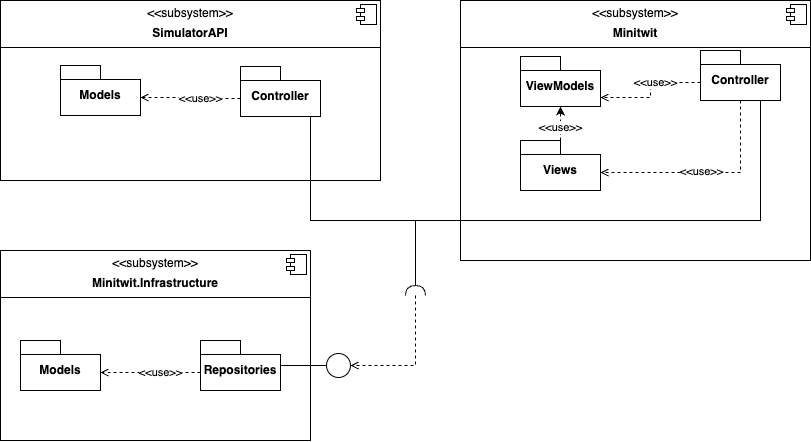
\includegraphics[width=1\textwidth]{Subsystem-Interaction.png}
    \end{center}
    \caption{An overview of the subsystems and how they interact}
    \label{fig:subsystem-interaction}
\end{figure}

Because the two main subsystems are inherently different we wanted to implement a database abstraction layer such that we had a uniform way of querying the database. Therefore, both controllers use the Repository package from the subsystem Minitwit.Infrastructure to query the database using the Repository pattern\cite{repo_pattern}.
%cite
Due to the different specifications for the Minitwit and SimulatorAPI, the controller for Minitwit is more complex. As can be seen in figure \ref{fig:frontend-interaction} the controller for Minitwit has to present information in a GUI, whereas the SimulatorAPI only calls the repository to fetch the user messages, as can be seen in figure \ref{fig:backend-interaction}.
\begin{figure}[H]
    \begin{center}
        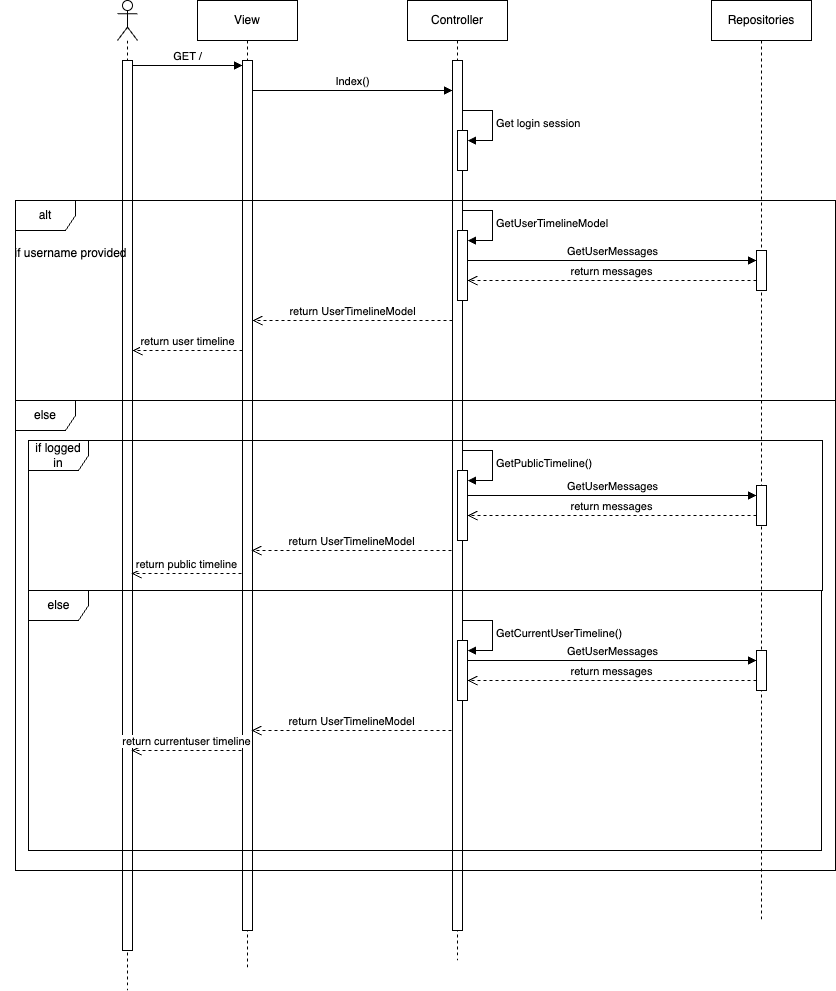
\includegraphics[width=1\textwidth]{Fronted-Sequence-Diagram.png}
    \end{center}
    \caption{Minitwit: Sequence diagram of a user call to the index page}
    \label{fig:frontend-interaction}
\end{figure}
\begin{figure}[H]
    \begin{center}
        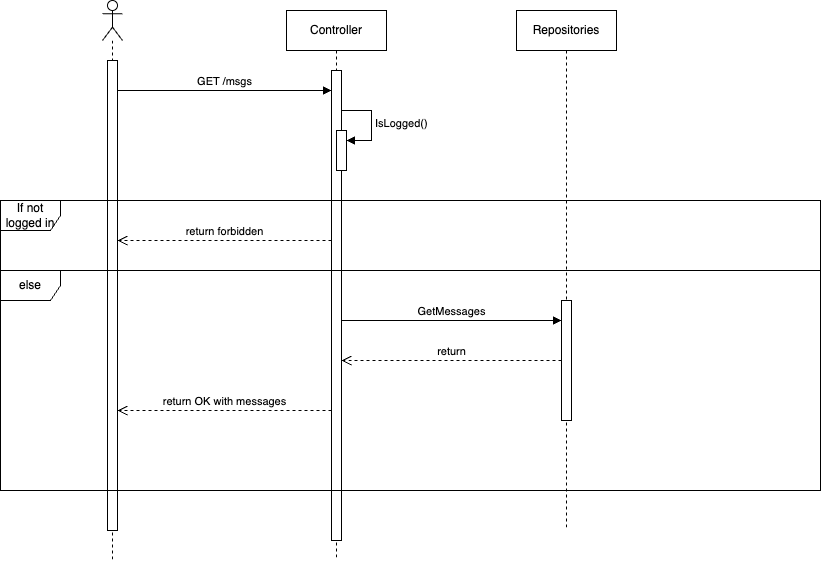
\includegraphics[width=1\textwidth]{Backend-Sequence-Diagram.png}
    \end{center}
    \caption{SimulatorAPI: Sequence diagram of a user call to get messages}
    \label{fig:backend-interaction}
\end{figure}


\subsection{Current state}
Table \ref{current-table} describes the status of the system after the simulator has been shut down.
\begin{table}[H]
    \begin{center}
        \begin{tabular}{ |c|c| }
            \hline
            Total requests & 34233 \\
            \hline
            Requests secured & 34233 \\
            \hline
            Total unhandled exceptions & 18 \\
            \hline
            P99 min response time & 94.2 ms \\
            \hline
            P99 max response time & 716 ms \\
            \hline
            Number of users &  116995\\
            \hline
            Avg followers per user &  28.5\\
            \hline
        \end{tabular}
    \end{center}
    \caption{System metrics}
    \label{current-table}
\end{table}
Furthermore, the static analysis tool Sonarcloud assesses that the quality of the overall code is good (see appendix \ref{appendix:sonarcloud}).
